\section{Rendering in Filmen}
\subsection{Abstrakt}
\label{sec:renderingAbstrakt}
Rendering bezeichnet im Allgemeinen das Erstellen eines zweidimensionalen Bildes aus einer dreidimensionalen Szene oder eines Objektes unter Ber�cksichtigung physikalische Gr��en wie Licht, Schatten und Materialien \cite{renderingDefinition}. Dieser Prozess findet in einer Vielzahl von unterschiedlichen Bereichen Anwendungsf�lle. Zum einen in der Darstellung von Computerspielen, bei Konstruktionen in CAD-Programmen aber auch bei CGI in aktuellen Filmen. 
Jeder Anwendungsfall hat andere Anforderungen und Priorit�ten an das Rendering. W�hrend Computerspiele vor Allem ein schnelles Erzeugen von Bildern ben�tigen, kommt es in Filmen auf eine m�glichst reale und detailreiche Darstellung an. Das folgende Kapitel besch�ftigt sich mit den besonderen Anforderungen an das Rendering im Film. Hierbei wird sowohl die Erstellung komplett synthetischer Filme wie Cars~\ref{cars} oder Monster AG als auch das Einbetten synthetischer Objekte in reale Bilder betrachtet.

\begin{figure}[t]
	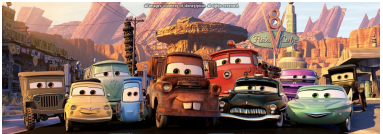
\includegraphics[width=13cm]{02_Rendering/img/cars.png}
	\caption[Bild aus dem Film Cars]{Bild aus dem Film Cars. Entnommen aus \cite{cars}}
	\label{cars}
\end{figure}

\subsection{Einf�hrung}
Die Anforderungen an das Rendering in Filmen sind vielf�ltig. Die Bilder m�ssen in einer angemessenen Zeit gerendert werden und trotzdem einen hohen Detailgrad aufweisen. Zus�tzlich m�ssen sich Licht und Materialien im Filmkontext korrekt verhalten um dem Betrachter das Gef�hl einer realistischen Szene zu geben. Das hei�t es m�ssen Reflexionen, Brechungen von Licht, sowie Schatten und Materialeigenschaften wie Transparenz ber�cksichtigt werden. All das kann bereits bei relativ kleinen Objekten zu aufwendigen Berechnungen f�hren. Beim Film arbeiten wir jedoch mit sehr komplexen Szenen, welche aus vielen Objekten bestehen. Aus diesen Szenen m�ssen f�r eine Sekunde Film 24 hochaufl�sende Bilder erstellt werden. Im folgenden werden zun�chst grundlegende Eigenschaften von Beleuchtung und Materialien er�rtert, um dann unter Ber�cksichtigung der oben genannten Anforderungen, auf die Erzeugung einer komplett synthetischen Szene als auch das Einf�gen eines synthetischen Charakters in eine reale Szene einzugehen.

\subsection{Licht}
Jede Rendering Technik versucht das gleiche physikalische Ph�nomen abzubilden. N�mlich die Streuung von Licht \cite{renderingEquation}. Wie viel Licht sich an einem Punkt im Raum befindet ergibt sich zum einen aus dem direkt von einer Lichtquelle einfallenden Licht, als auch durch das Licht, welches von umliegenden Punkten auf den Punkt reflektiert wird. Diese beiden Faktoren werden mit Hilfe lokaler Reflexionsmodelle beziehungsweise Globaler Beleuchtungsmodelle angen�hert. Aktuelle Rendering Techniken bedienen sich sowohl der lokalen Reflexions- als auch globaler Beleuchtungsmodelle.

\subsubsection{Lokale Reflexionsmodelle}
Alan Watt beschreibt in seinem Buch 3D Computergrafik lokale Reflexionsmodelle als eine M�glichkeit den Betrag der direkten Beleuchtung an einem Punkt zu ermitteln \cite{localLight}. Dieser Wert wird durch eine Bi-Directional Reflection Distribution Function (BRDF) kategorisiert. Dabei wird Anhand der Richtung der einfallenden Lichtstrahlen   

\begin{equation}
\label{formel}
f_{i,j}=
\sum_{x=0}^{N-1} \sum_{y=0}^{N-1}
\frac{2 \cdot C(x)\cdot C(y)}{N} \cdot 
F_{x,y} \cdot 
\cos \left( \frac{(2i+1) \cdot x \cdot \pi}{2 \cdot N} \right) \cdot
\cos \left( \frac{(2j+1) \cdot y \cdot \pi}{2 \cdot N} \right)
\end{equation}
Formeln im Flie�text binden sich sehr einfach ein. So kann man den
bekannten Pythagoras schreiben als $a^2 + b^2 = c^2$. F�r die gleiche
Formel wie (\ref{formel}) ohne automatische Nummerierung erh�lt man,
indem man die Umgebung, in der sie sich befindet, anpasst:

\[
f_{i,j}=
\sum_{x=0}^{N-1} \sum_{y=0}^{N-1}
\frac{2 \cdot C(x)\cdot C(y)}{N} \cdot 
F_{x,y} \cdot 
\cos \left( \frac{(2i+1) \cdot x \cdot \pi}{2 \cdot N} \right) \cdot
\cos \left( \frac{(2j+1) \cdot y \cdot \pi}{2 \cdot N} \right)
\]


Abs�tze werden durch Leerzeilen abgegrenzt.

